\documentclass[12pt]{article}

\usepackage[utf8x]{inputenc}
\usepackage[spanish, es-lcroman]{babel}

\usepackage[final]{pdfpages} %para insertar pdfs


\usepackage{amssymb,amsmath,amsthm,amsfonts}
\usepackage{calc}
\usepackage{graphicx}
\usepackage{subfigure}
\usepackage{textcomp}
\usepackage{gensymb}
\usepackage{natbib}
\usepackage{url}
\usepackage[utf8x]{inputenc}
\usepackage{amsmath}
\usepackage{graphicx}
\graphicspath{{images/}}
\usepackage{parskip}
\usepackage{fancyhdr}
\usepackage{vmargin}
\usepackage[colorlinks=true, linkcolor=black, urlcolor=blue, pdfborder={0 0 0}]{hyperref}
\setmarginsrb{3 cm}{2.5 cm}{3 cm}{2.5 cm}{1 cm}{1.5 cm}{1 cm}{1.5 cm}

\title{Informe Trabajo Práctico Final}					% Titulo
\author{Pablo}					% Autor
\date{\today}						% Fecha


\makeatletter
\let\thetitle\@title
\let\theauthor\@author
\let\thedate\@date
\makeatother

\pagestyle{fancy}
\fancyhf{}
\rhead{\theauthor}
\lhead{\thetitle}
\cfoot{\thepage}


%%%%%%%%%%%%%%%%%%%%%%%%%%%%%%%%%%%%%%%%%%%%%%%%%%%%%%%%%%%%%%%%%%%%%%%%%%%%%%%%%%%%%%%%%

\usepackage{listings}
\usepackage{color}

\definecolor{dkgreen}{rgb}{0,0.6,0}
\definecolor{gray}{rgb}{0.5,0.5,0.5}
\definecolor{mauve}{rgb}{0.58,0,0.82}

\lstset{frame=tb,
  language=Java,
  aboveskip=3mm,
  belowskip=3mm,
  showstringspaces=false,
  columns=flexible,
  basicstyle={\small\ttfamily},
  numbers=none,
  numberstyle=\tiny\color{gray},
  keywordstyle=\color{blue},
  commentstyle=\color{dkgreen},
  stringstyle=\color{mauve},
  breaklines=true,
  breakatwhitespace=true,
  tabsize=3
}

%%%%%%%%%%%%%%%%%%%%%%%%%%%%%%%%%%%%%%%%%%%%%%%%%%%%%%%%%%%%%%%%%%%%%%%%%%%%%%%%%%%%%%%%%






\begin{document}

%%%%%%%%%%%%%%%%%%%%%%%%%%%%%%%%%%%%%%%%%%%%%%%%%%%%%%%%%%%%%%%%%%%%%%%%%%%%%%%%%%%%%%%%%

\begin{titlepage}
	\centering
    \vspace*{0.0 cm}
    
\includegraphics[scale = 0.7]{Universidad_Nacional_de_Cordoba.png}\\[1.0 cm]	% Logo Universidad
    \textsc{\LARGE Universidad Nacional de Córdoba}\\[1.5 cm]	% Nombre Universidad
	\textsc{\Large Programación Concurrente}\\[0.5 cm] %departamento
	%\textsc{\large CC4901 Práctica Profesional II}\\[0.5 cm]% Codigo y Nombre Curso
	\rule{\linewidth}{0.2 mm} \\[0.4 cm]
	{ \huge \bfseries \thetitle}\\
	\rule{\linewidth}{0.2 mm} \\[1.5 cm]
	
\centering
\begin{tabular}{ll}
Alumnos:			&	Nombre de alumno 1, (Código)\\
					&	Nombre de alumno 2, (Código)\\
Profesor:			&	Dr. xxxxxxx
\end{tabular}	
	
	
	\begin{minipage}{0.4\textwidth}
		\begin{flushleft}
	
		\end{flushleft}
	\end{minipage}
	\begin{minipage}{0.4\textwidth}
		\begin{flushleft} \large
			\theauthor \\
        
          {\small xxxxxx@mi.unc.edu.ar}\\ %email
          %{\small (+56) 9 XXXX XXXX} %teléfono
		\end{flushleft}
	\end{minipage}~
	\begin{minipage}{0.4\textwidth}
		\begin{flushright} \large
			\emph{Matrícula} \\
			xxxxxx1	\\%nro de matricula	
            
           % {\Large Empresa u Organización} %Empresa u Organización donde se hizo la práctica
		\end{flushright}	
	\end{minipage}\\[2 cm]
	
	
	{\large \thedate}\\[2 cm]
 
	\vfill
	
\end{titlepage}
%%%%%%%%%%%%%%%%%%%%%%%%%%%%%%%%%%%%%%%%%%%%%%%%%%%%%%%%%%%%%%%%%%%%%%%%%%%%%%%%%%%%%%%%%
%\chapter*{\LARGE \textbf{Observaciones}} %página siempre en blanco
%\pagenumbering{Roman}
\pagenumbering{gobble}



\section*{Resumen}


\newpage
%%%%%%%%%%%%%%%%%%%%%%%%%%%%%%%%%%%%%%%%%%%%%%%%%%%%%%%%%%%%%%%%%%%%%%%%%%%%%%%%%%%%%%%%%

\tableofcontents %% indice

\pagebreak
\pagenumbering{arabic}
\section{Introducción}
  
\pagebreak
%%%%%%%%%%%%%%%%%%%%%%%%%%%%%%%%%%%%%%%%%%%%%%%%%%%%%%%%%%%%%%%%%%%%%%%%%%%%%%%%%%%%%%%%%
\section{Desarrollo}
\subsection{Red de Petri}
\subsubsection{Verificación de las Propiedades}
\subsection{Cantidad de Hilos}
\subsection{Políticas}
\begin{lstlisting}
// Hello.java
import javax.swing.JApplet;
import java.awt.Graphics;

public class Hello extends JApplet {
    public void paintComponent(Graphics g) {
        g.drawString("Hello, world!", 65, 95);
    }    
}
\end{lstlisting}
\subsubsection{Equidad de las Políticas}
\subsection{Análisis de Invariantes}
\subsubsection{P-Invariantes}
\subsubsection{T-Invariantes}


%%%%%%%%%%%%%%%%%%%%%%%%%%%%%%%%%%%%%%%%%%%%%%%%%%%%%%%%%%%%%%%%%%%%%%%%%%%%%%%%%%%%%%%%%
\pagebreak
\section{Diagramas}
\subsection{Diagrama de clase}{
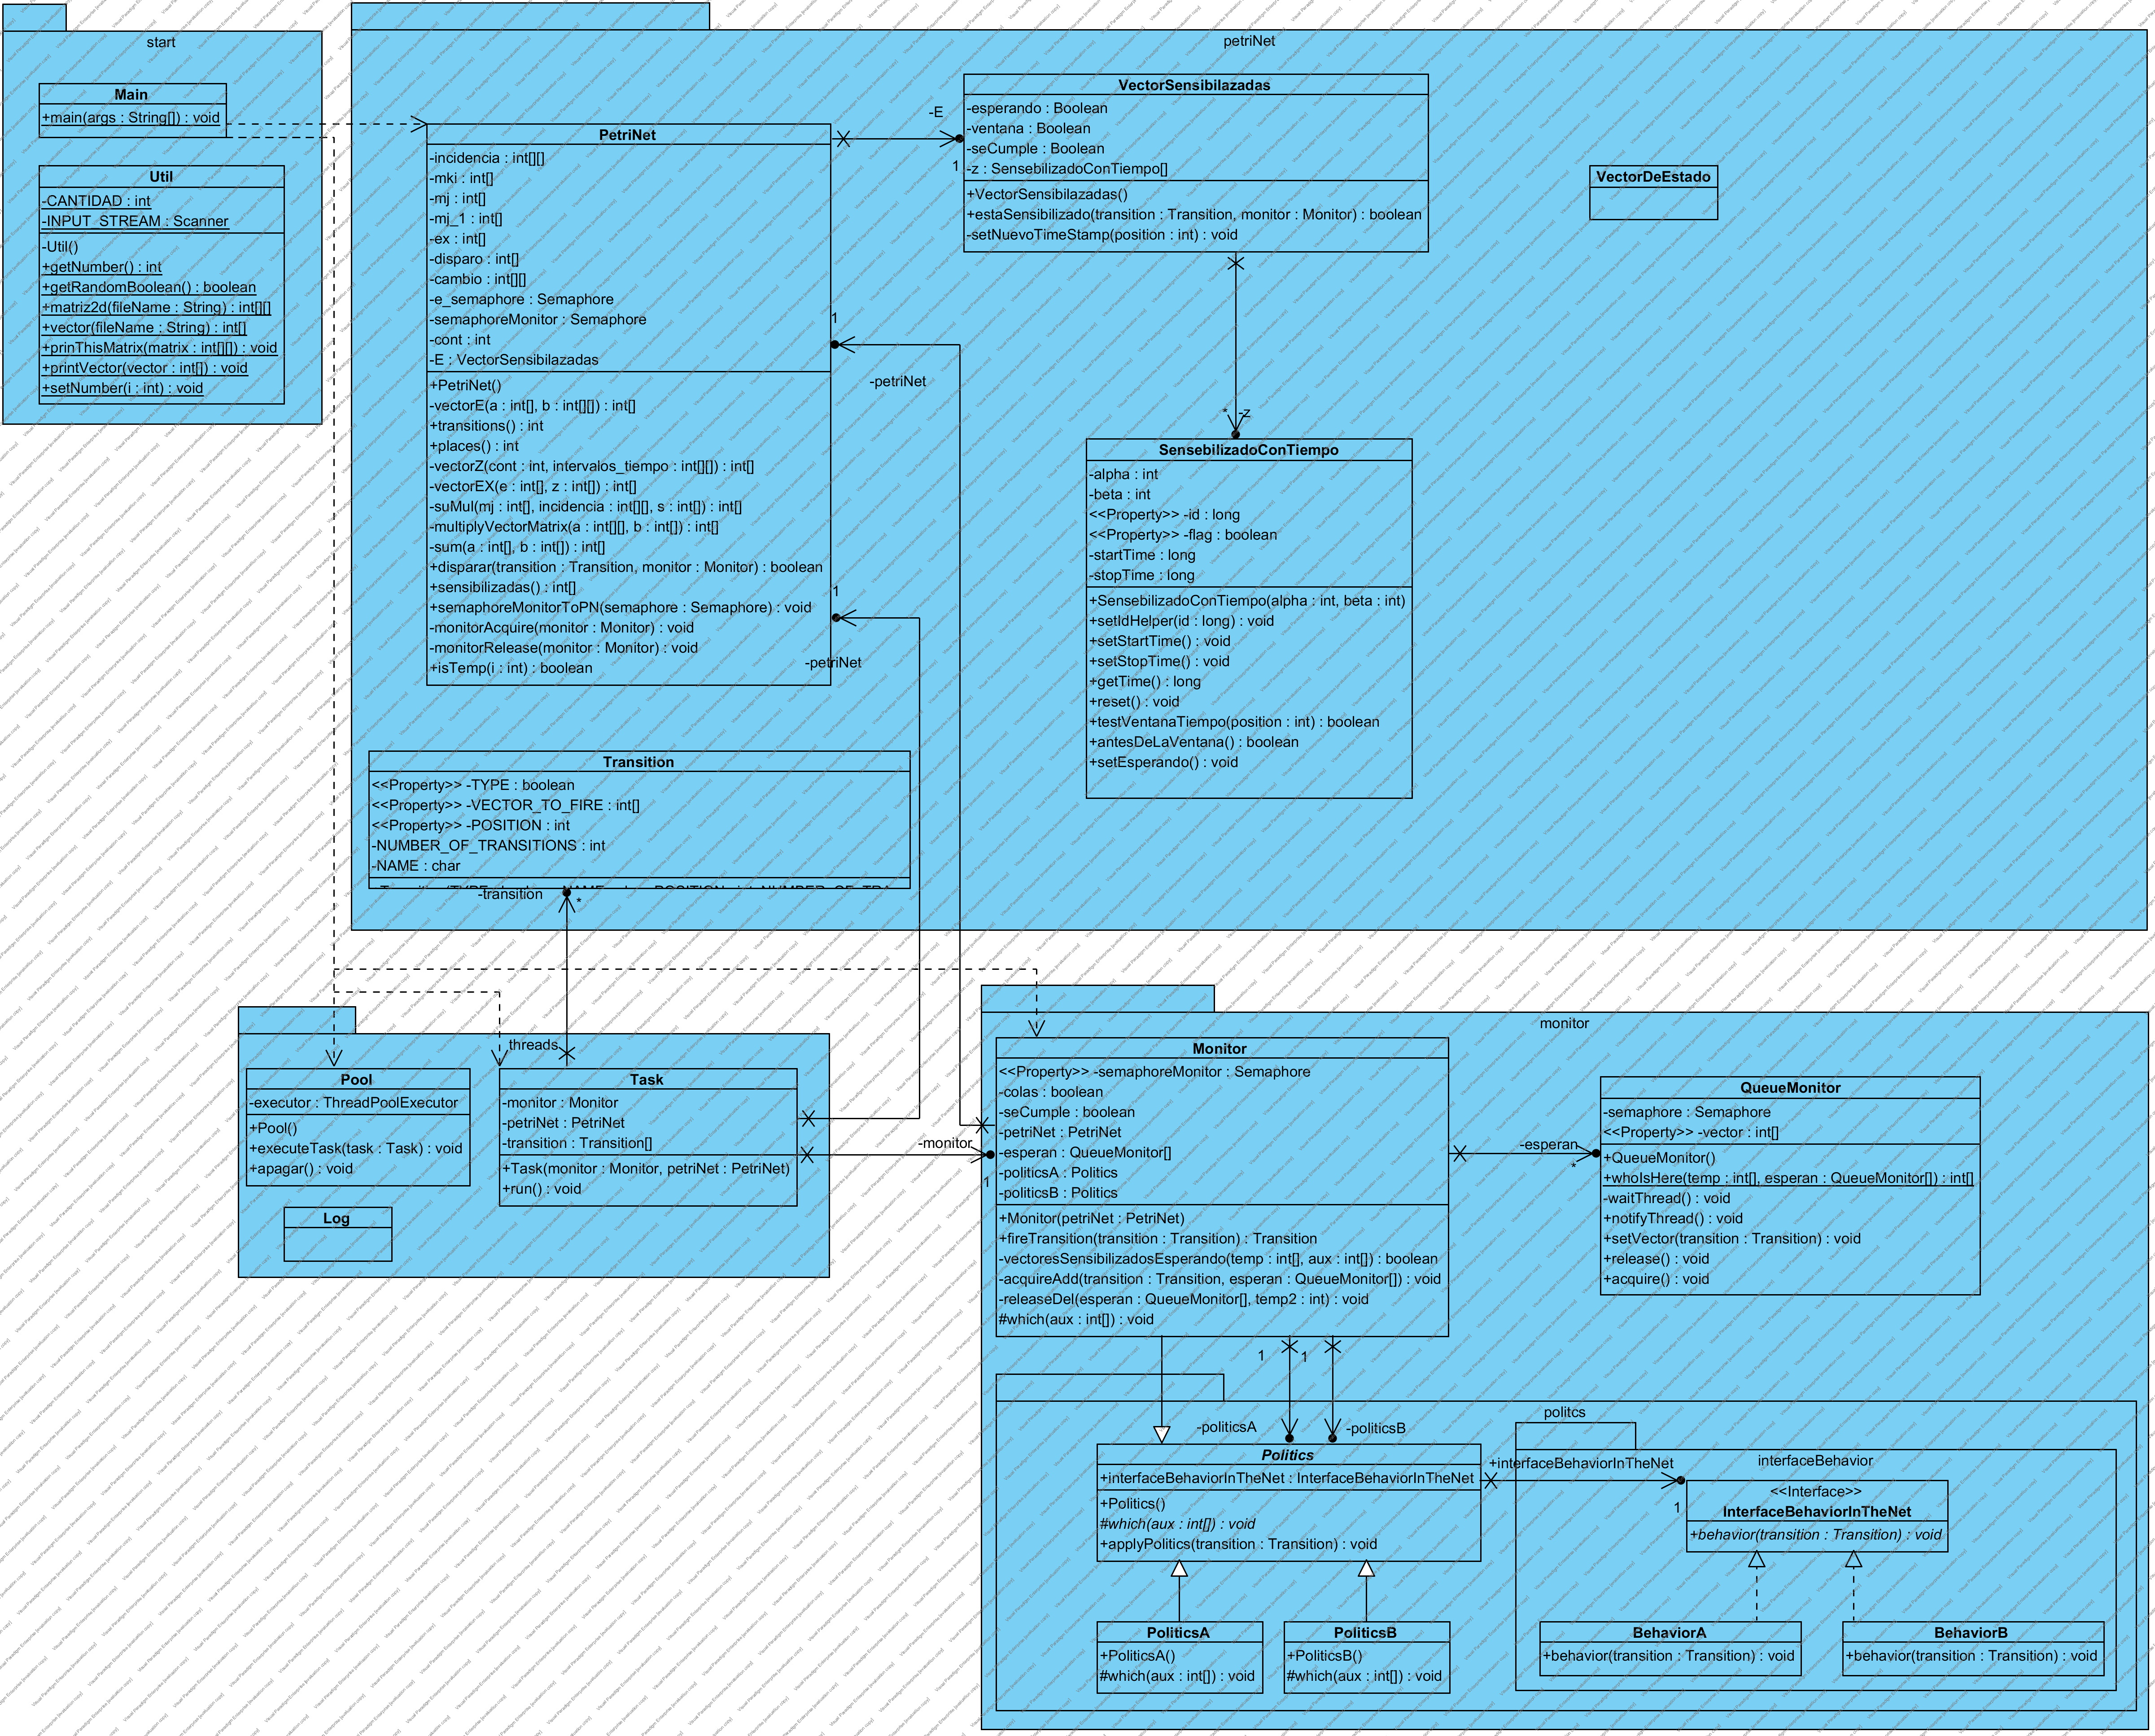
\includegraphics[width=\textwidth,height=\textheight,keepaspectratio]{Diagrama_Clase.png}
%scan del formulario de evaluación
%{
%\includepdf[pages=1,pagecommand={},offset=2.5cm -1cm]{Class_Diagram.pdf} %pdf
%\includegraphics[scale = 0.9]{form.png}\\[1.0 cm]%imagen
%}
\pagebreak

}
\subsection{Diagrama de secuencia del disparo de una transicion}
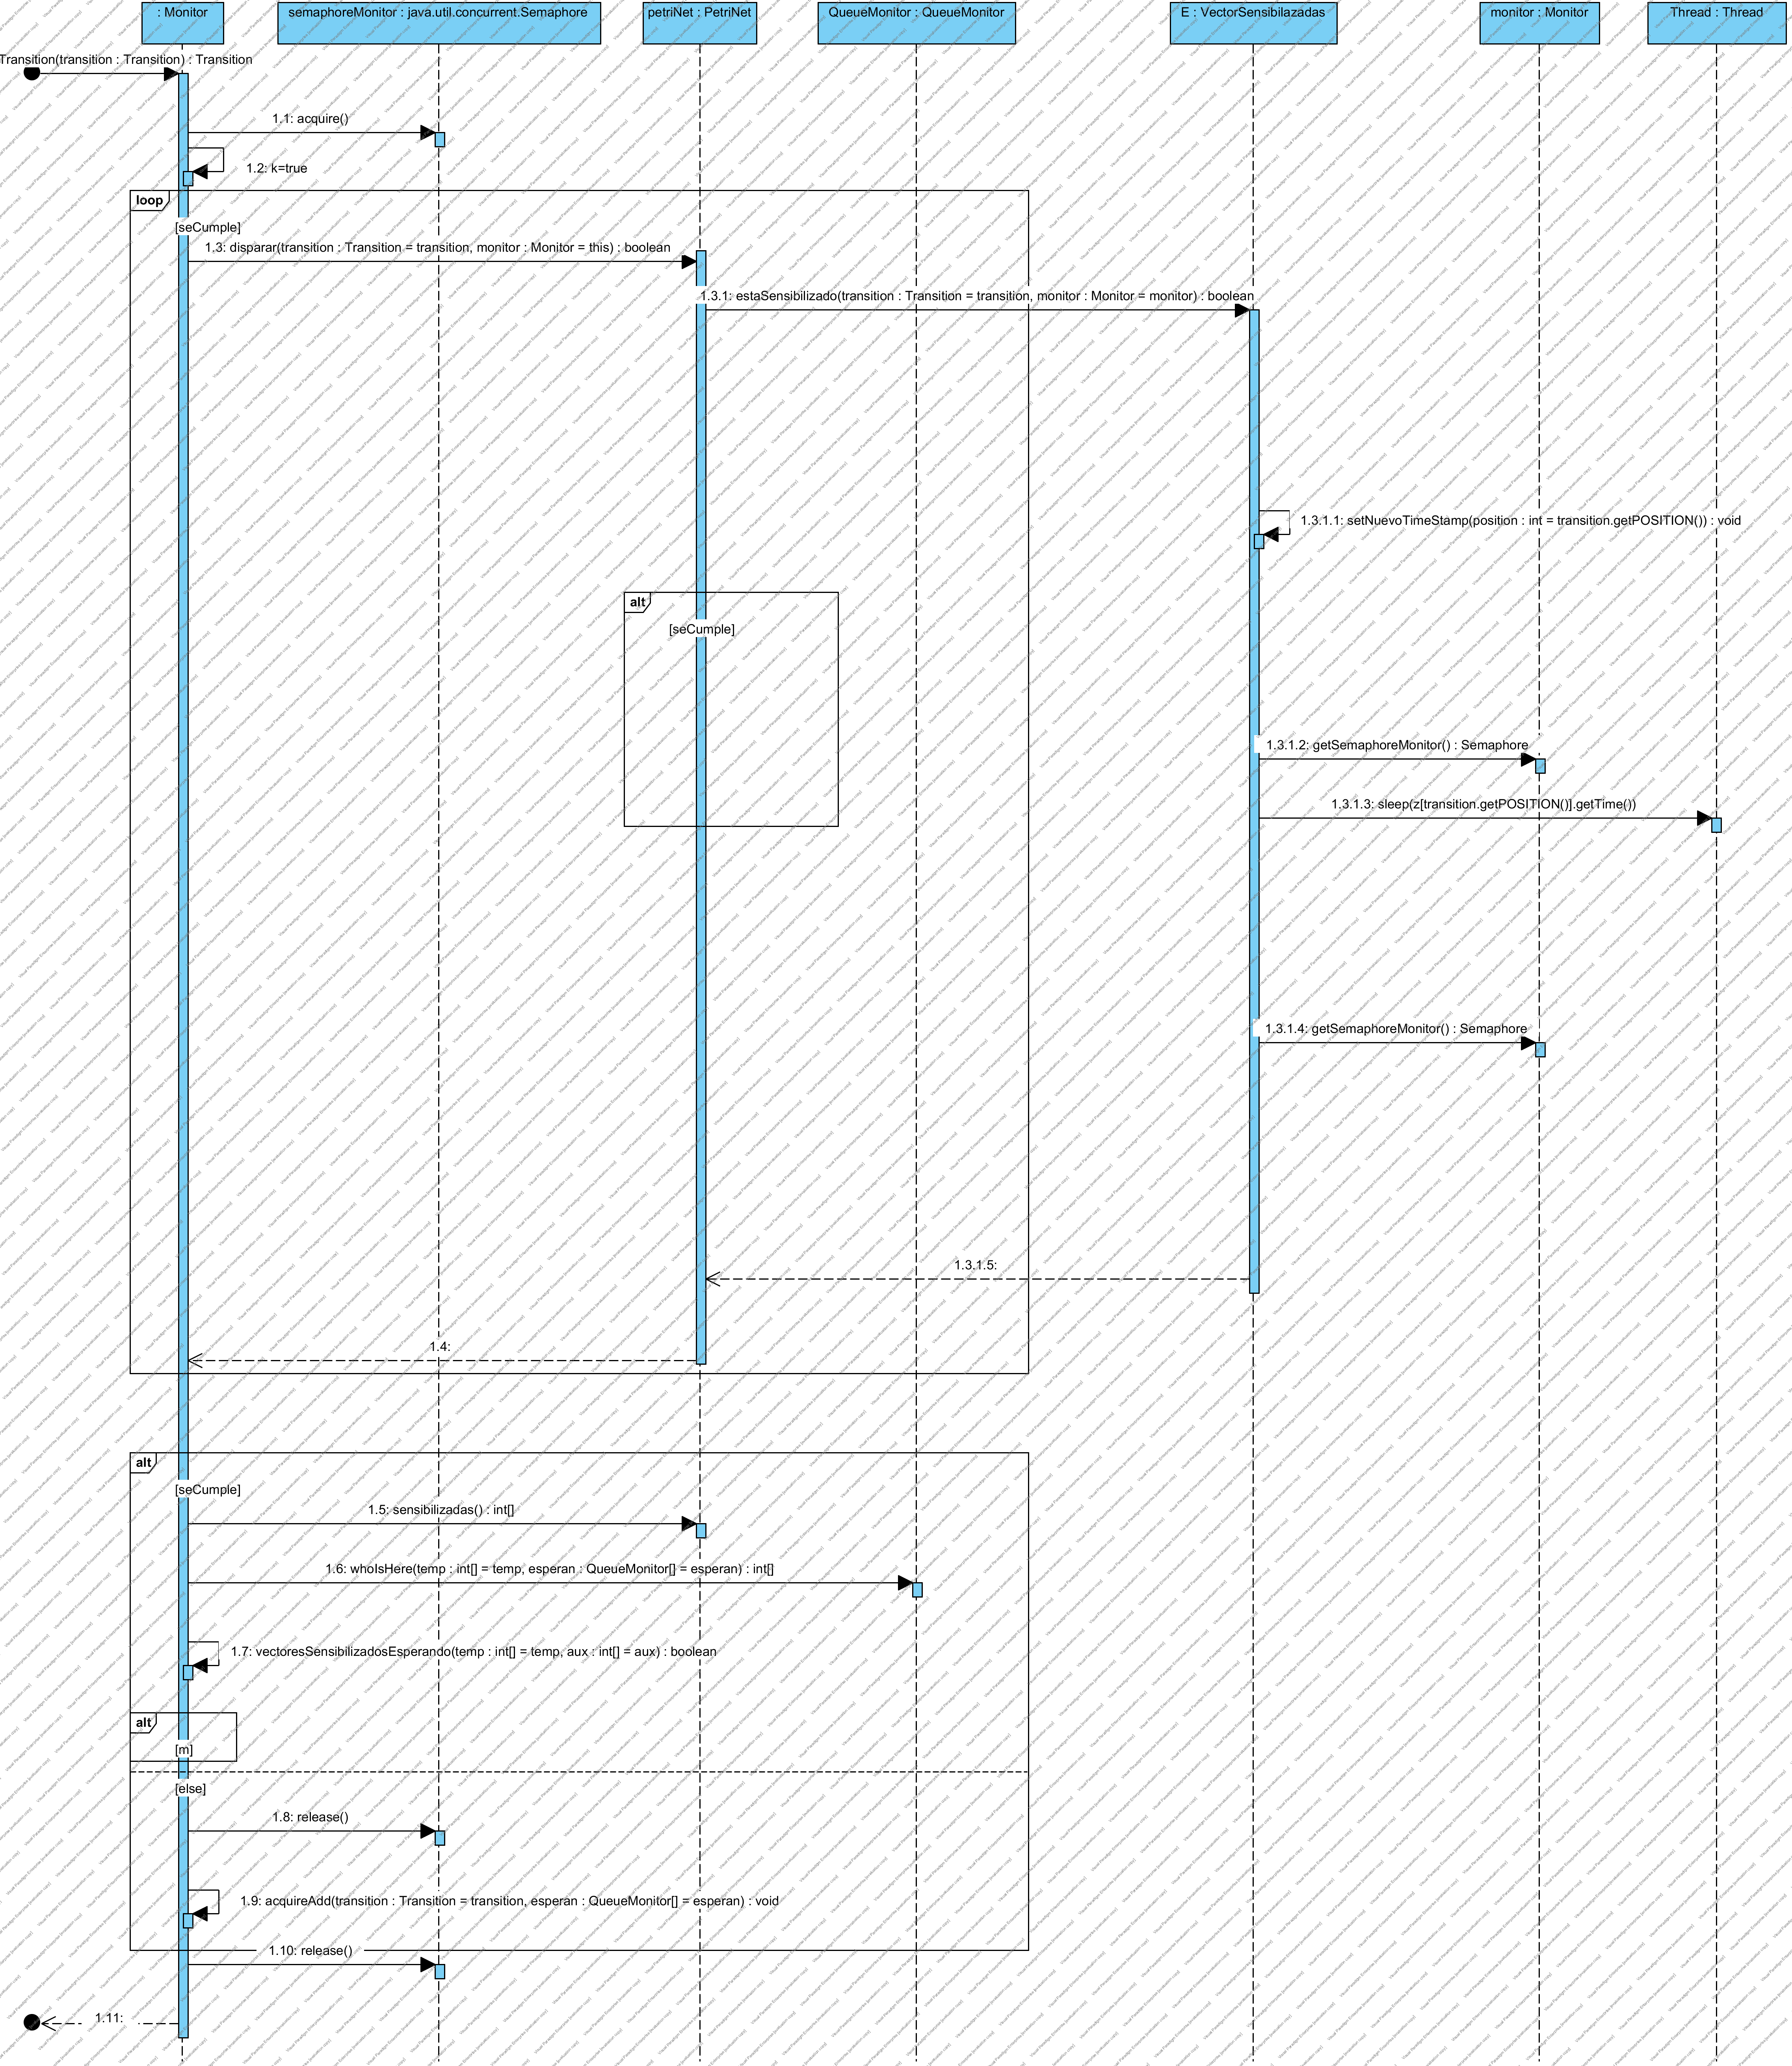
\includegraphics[width=\textwidth,height=\textheight,keepaspectratio]{Secuencia_Transicion.png}
\pagebreak
%%%%%%%%%%%%%%%%%%%%%%%%%%%%%%%%%%%%%%%%%%%%%%%%%%%%%%%%%%%%%%%%%%%%%%%%%%%%%%%%%%%%%%%%%
\section{Conclusión}
\pagebreak

\end{document}
